\chapter{Background} \label{ch:[chapter 2 label]}

In this section, I discuss important background for my research. This includes details about cognitive processes, like formulating \gls{information_need}s, resulting user search behaviors, and how a search system technically attempts to interpret user requests. To give an overview of the IR process, figure \ref{fig:Background_Complete_Search_System}. depicts the components of a complete search system. The IR  process is both cognitively and technically complex, therefore I have summarized the important steps for my research in figure \ref{fig:Background_IR_Steps}. For further details on IR, I refer readers to comprehensive literature on user needs and interactions while searching \cite{White2016}, modern IR system architectures \cite{Baeza-Yates1999}, and IR data structures and algorithms including the vector space model and relevance feedback \cite{Buckley1985}.

\begin{figure}
    \centering
    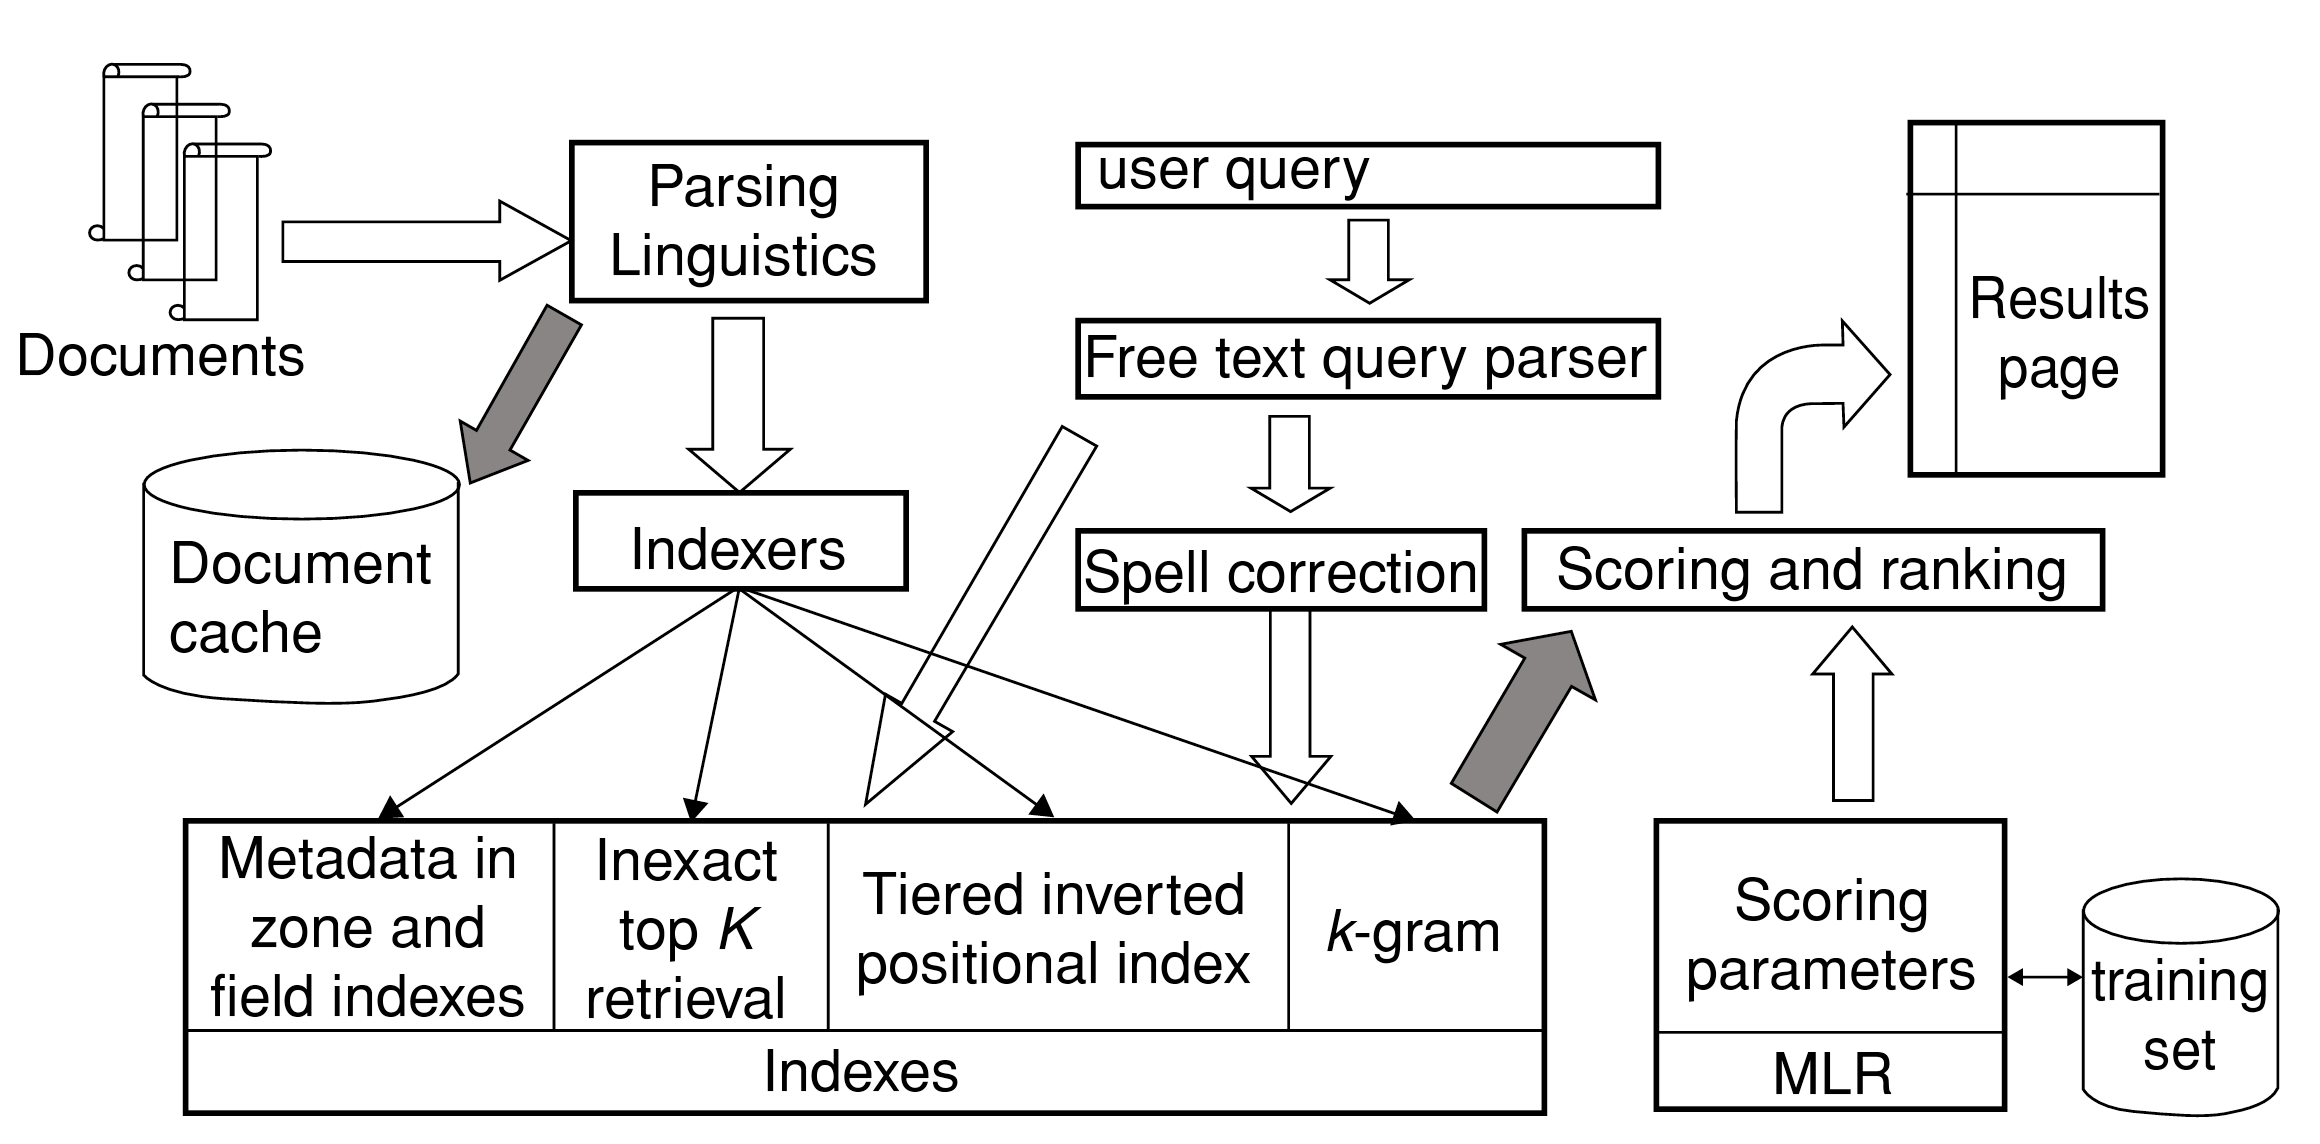
\includegraphics[width=1\textwidth]{../figures/Background_Complete_Search_System.png}
    \caption{This figure, borrowed from \cite{Manning2008}, depicts a complete search system. On the left side of the figure, documents are parsed an indexed to be retrieved. In the center, a user’s query is ingested and parsed. On the right, scoring parameters are used to compare a parsed query and indexed document representations. Documents are assigned a final composite score calculated by linearly combining similarity scores between documents and a query for multiple criteria. The output is a ranked list of results on a page typically called a search engine results page (SERP).}
    \label{fig:Background_Complete_Search_System}
\end{figure}

\begin{figure}
    \centering
    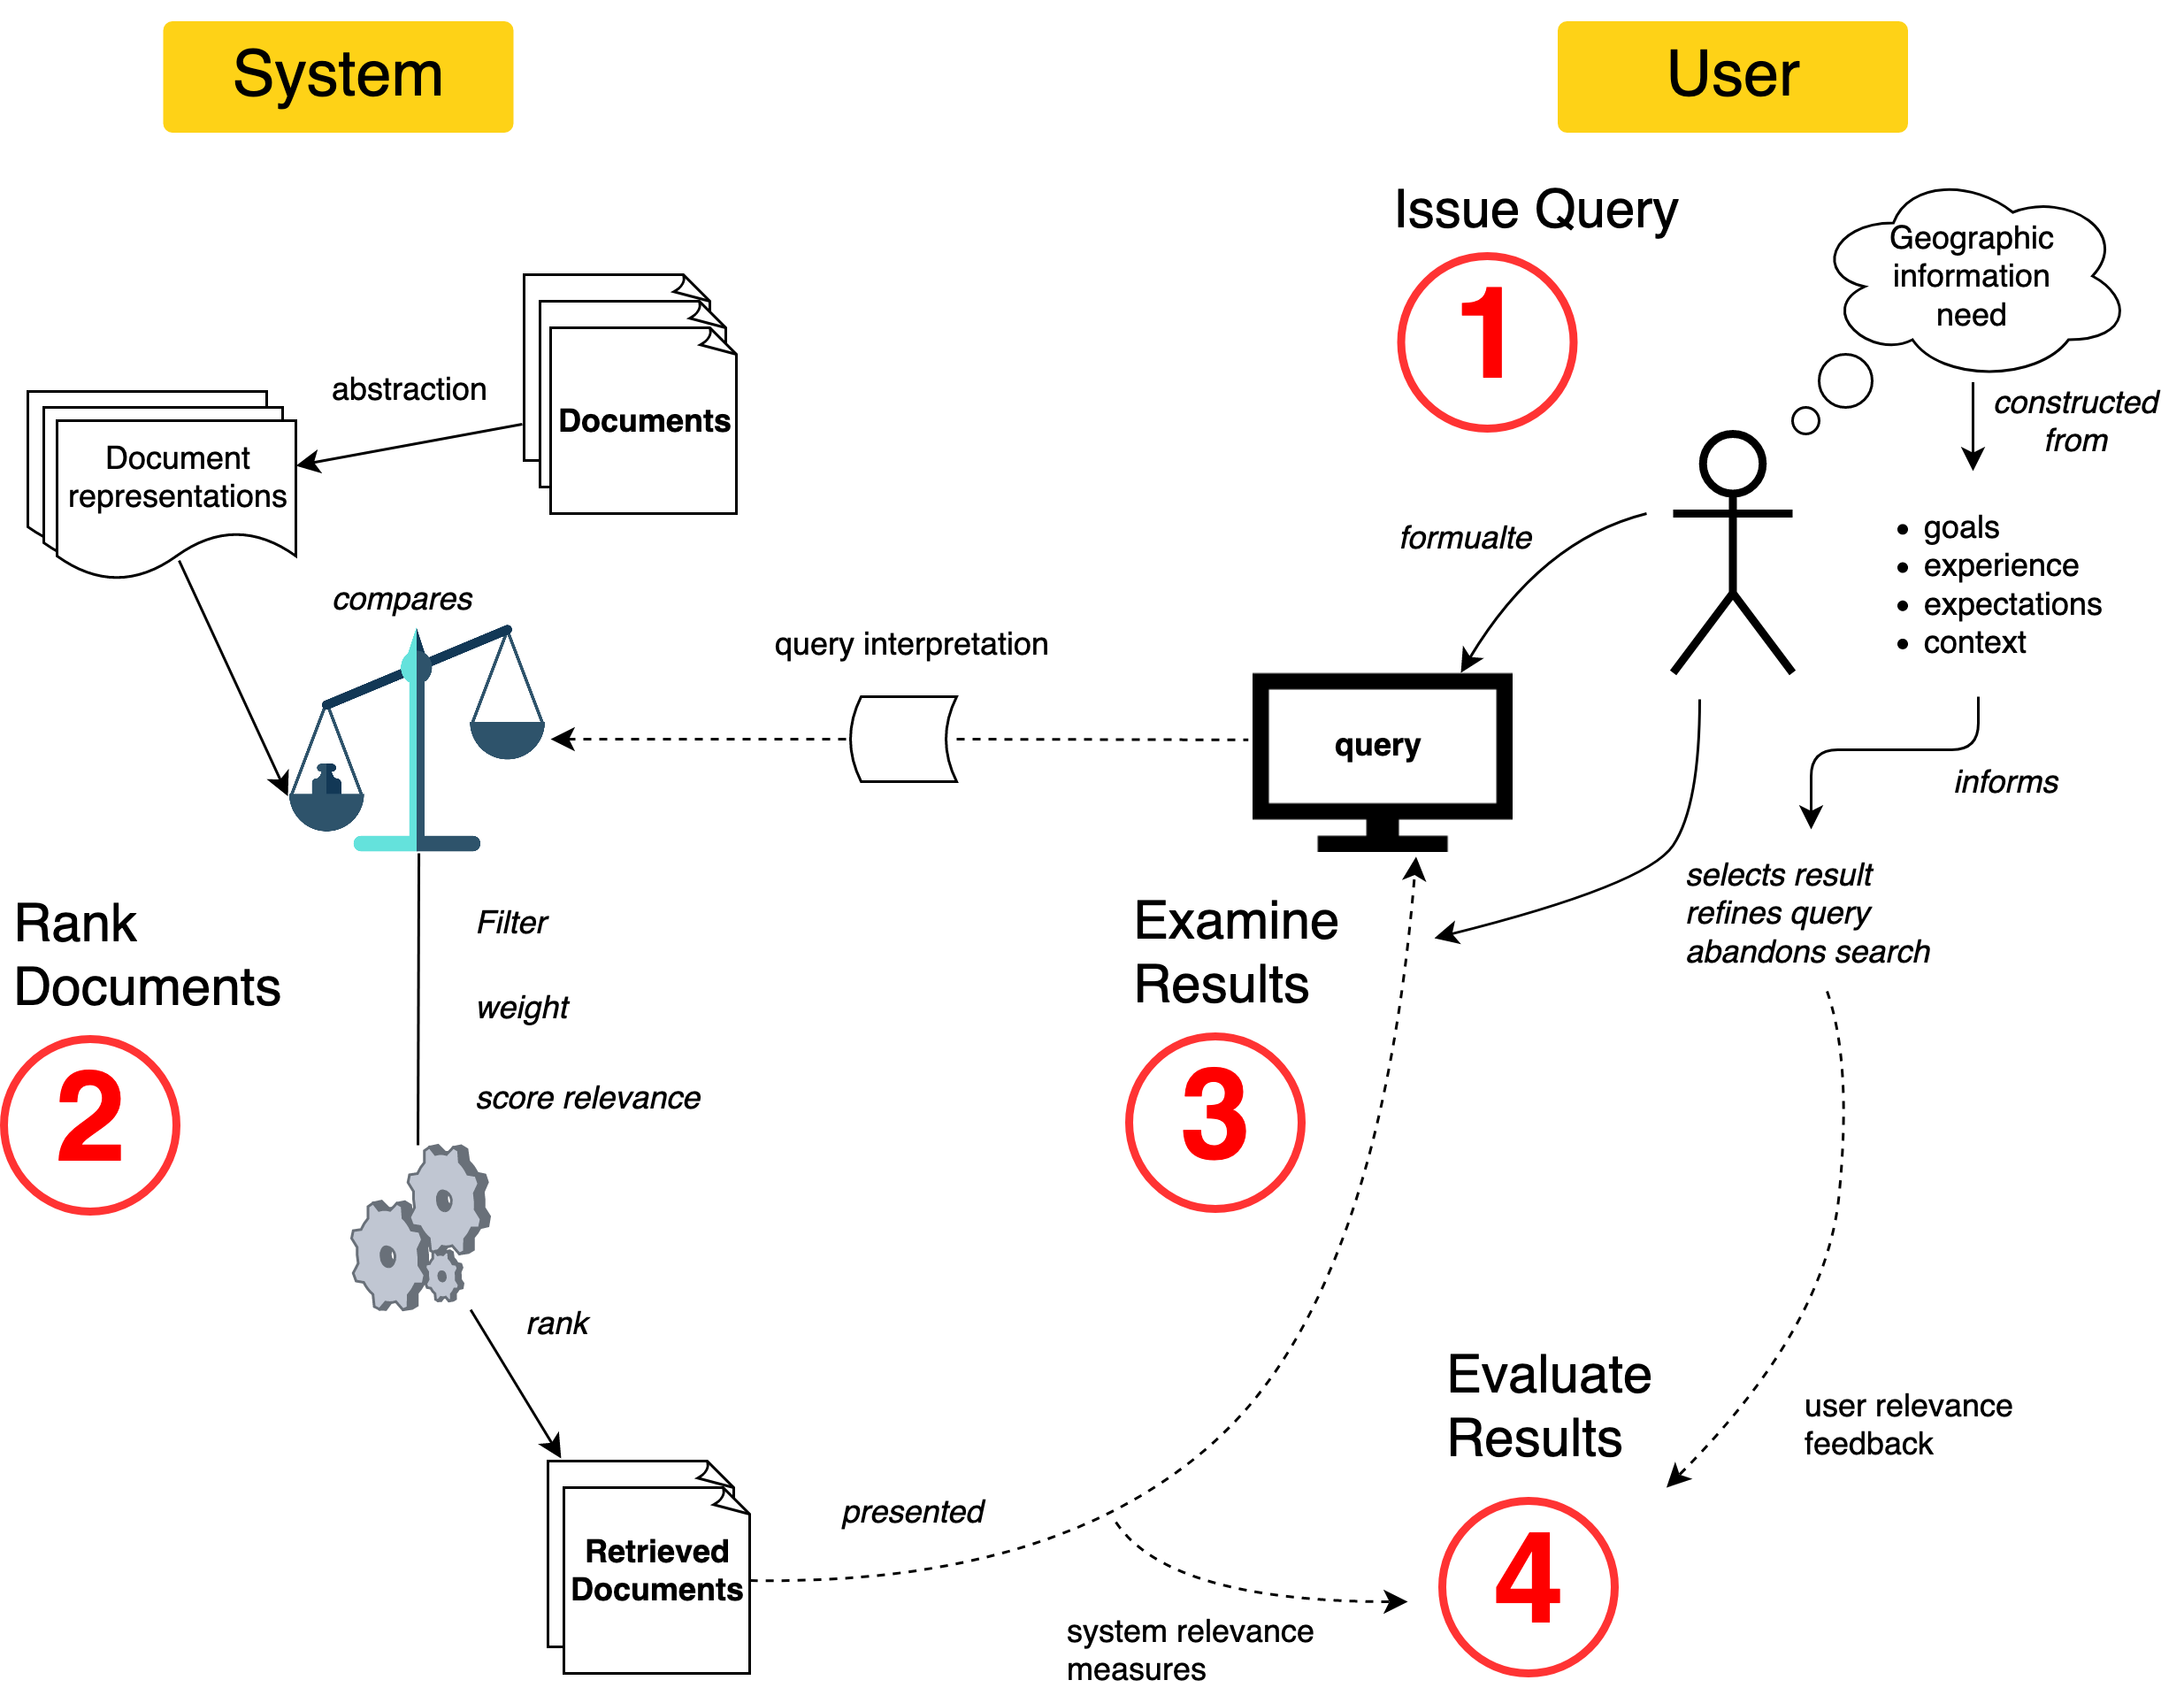
\includegraphics[width=1\textwidth]{../figures/Background_IR_Steps.png}
    \caption{A simplified overview of the IR process with emphasis on steps important to this study. Dashed lines represent information transfers and italics represent actions. Step 1: User formulates and issues a query based on GINs. Step 2: Search system compares document representations and a query interpretation and ranks documents by relevance. Step 3: Resulting documents are ordered, presented, and examined by the user. Users then select and explore results, refine their query, or abandon search. Step 4: A system is evaluated for effectiveness based on user relevance feedback and/or system relevance measures including precision, recall, MAP, and NGDC, among others. See glossary for measure definitions.}
    \label{fig:Background_IR_Steps}
\end{figure}

\section{Geographic Information Needs of Data Searchers}

Geographic information needs of data searchers are diverse, uncertain, hard to describe and hard to articulate. Overall, diverse needs are driven by diverse questions that in turn drive particular \gls{information_seeking} activities and strategies. Some users have targeted searches, like finding a datasets on crime, while others browse available datasets either out of curiosity or in hopes of discovering something new and useful. In text-based search, some users express needs using natural language while others use keywords or topics. What is more, diverse needs yield even more diverse expectations. For example, users that perform a targeted search are typically seeking a specific type of information, but how that information is labeled, how it is presented, and its required contents are just a few possible expectations. Broadly speaking, the domain of IR studies information needs along with the "representation, storage, organization of, and access to information items such as documents, Web pages, online catalogs, structured and semi-structured records, [and] multimedia objects" \cite{Baeza-Yates1999}. IR attempts to structure and serve relevant resources to a user based on their articulated needs. 

User needs are not directly observable. So, the IR community studies user needs indirectly by observing user search behavior and asking users for feedback. In theory, someone who is engaged in an information seeking activity will give clues to their needs based on what they search for and how they search for it. For example, if someone searches for "tacos near me" on the Yelp platform at noon, to a human it can be reasonably inferred that this person wants to find a place for lunch that serves tacos. To accomplish this, they need information about restaurants. For computers, understanding this is a monumental task. IR systems must try to comprehend human language as humans do. Since IR systems cannot directly interpret user needs, they should try to interpret the next closest things, \emph{relevance}, \emph{usefulness}, and user \emph{satisfaction}.

\section{User Search Behavior}

Recording user search behavior is a critical step towards understanding user needs. Similar to observing people i a psychological study, observing how a user interacts with a search system provides many clues as to what they want to do, what they ended up doing, and what the system should do to be more effective. Search behavior is studied because relevance, usefulness, and satisfaction inferences can be made from particular behaviors. For example, broadly speaking, if a person uses a search tool and exits quickly or continually refines their search queries, then they haven't found an result that satisfies their needs. If they dwell on a result, it can be assumed that they are interested in that result. Once behavior is understood, researchers change the search system and then record the difference in behavior. For example, if changing a ranking algorithm rearranges the top search results, researchers can observe if users only select the top results or if they select the same results as before, indicating that those results are relevant.

Studying search behavior is not an easy task. For example, presentation biases on a search engine result page (typically called a \acrshort{SERP}) including positionality, authority, and visual appeal of results can attract users to certain results \cite{Hofmann2016}. There are also contextual factors that are hard to control for, such as a user's prior knowledge, their search environment, and their cognitive bias (i.e., favoring positive-sounding search results) \cite{Hofmann2016}. However, some broad behavior patterns have emerged. First, most users are somewhat impatient and use search tools quickly. After a few refinements, many will abandon the search session and seek information elsewhere. Second, users quickly navigate results. Many studies of \gls{query_logs}, the system records of user queries, clicks, and transactions, show that users will click on a result, return to the SERP, click on another result, return to the SERP, click on the first result again, etc. To a human, this pattern indicates that a user is comparing results, but to computers this behavior is often difficult to process. Third, the use of query keywords follows a power law and Zipf's law. Most query logs show that the same queries and query keywords are issued over and over with a very long tail of infrequent queries. This is important because a search system should make sure that it correctly handles the bulk of queries, especially if they're repeated, but also doesn't neglect the diverse needs of users. These patterns are a sample of user expectations, progressions, and articulations.

There are no IR research approaches that can completely control for individual search behaviors. Furthermore, the strength of the relationship between someone's information needs and their search behavior is subject to debate. Fortunately, controlled test collections have been developed for evaluating IR systems. Derived from the Cranfield studies, working groups at IR conferences like the Text Retrieval Conference\footnote{\url{https://trec.nist.gov/}} produce a collection of test query–document–relevance judgement triples that simulate users interacting with an IR system \cite{Sanderson2010} and selecting relevant documents. With a test collection, researchers change system components like relevance ranking, and evaluate if the changes are an improvement \cite{McGill1979}. This approach uses common system-oriented outcome evaluation measures to evaluate a system's effectiveness including \emph{\gls{precision}} (i.e., the percentage of selected results that are relevant), \emph{\gls{recall}} (i.e., the percentage of relevant results that are selected), \emph{\gls{mean_average_precision}} (\acrshort{mean_average_precision}) (i.e., precision across multiple queries), \emph{\gls{normalized_discounted_cumulative_gain}} (\acrshort{NDCG}) (i.e., graded relevance of a document based on its rank position). Human searchers, their behavior, and their interpretations are ignored.

Contrary to the system-oriented perspective, the user-oriented perspective tries to achieve a higher level of realism. This means that there is a higher focus on what users want out of a system, what results they find useful, and what ultimately satisfies them, not just how good a system is at retrieving the right results based on predefined relevance rules. This research approach evaluates a system using process-oriented evaluation measures. This means that it attempts to evaluate how a user feels during the search process based on search behavior and feedback through post-search surveys. Overall, both the system-oriented and user-oriented perspectives have their benefits and limitations.

% This approach typically issues post-search surveys where users rate either the usefulness or relevance of individual results, their query-level and task-level satisfaction, and other qualitative measures like frustration and happiness.

% In the next section, I discuss these limitations, an alternative approach, and the unique concept of geographic relevance.

\section{Relevance and Geographical Relevance}

As our information needs continue to grow, so will our demand for intuitive search tools build on robust IR systems. It's impractical to simply index more data and expect users to find the right answer by sifting through heaping results. Systems need to better interpret what results a user considers relevant.

% In the grand scheme of human needs, \emph{information needs} are arguably the easiest to satisfy. But
% Every day, humans must satisfy a multitude of needs from eating enough food to learning new job skills to entertaining themselves. Many times, humans don't know exactly what their needs are or how to articulate them, which is a problem that extends well into cognitive and behavioral sciences. 

In broad terms, relevance is the relation between user needs and what can be served by the entire information ecology \cite{Hjorland2010}. But relevance is heavily context dependent. For example, relevance can mean different things depending on judges (e.g., their biases, their error preferences), requests (e.g., diversity of content, specificity), documents (e.g., aboutness, recency), IR system usability (e.g., response speed, browsability), judgement conditions (e.g., breadth of document set, order of presentation), and choice of scale (e.g., kind of response required by user) \cite{Schamber1994}. Fortunately, in my research, search context is somewhat limited because document type and use are limited to the geospatial domain.

Hjørland effectively summarizes the broad views for studying relevance \cite{Hjorland2010}. The \emph{system} view is purely system-oriented and practically user need agnostic. It is interested in algorithmic relevance, perfectly matching documents to a query. This view is very common but criticized because analysis requires manual evaluations (e.g., binary relevance judgements made by an expert and/or on the fly graded user feedback) and subjectivity is clearly inherent in many design and evaluation choices.

Alternatively, the \emph{user} view "considers relevance to be a subjective individualized mental experience that involves cognitive restructuring" \cite{Borlund2003}(p. 914). Through this view, studying and psychologizing real users is preferred and their eventual satisfaction with results should be the motivator for system design. This view has become popular in recent years. However, Hjørland suggests that the user view has faults as well including often being positivist, lacking reflexivity, somewhat atheoretical and ignoring causal relationships, and suffering from the paradox that relevance is individual but researchers seek general tendencies. 

% Another view, the scholarship view, is typically criticized for being too narrow, concerns relevance to be purely based on scholarly arguments. Something is relevant if it "enable[s] and enhance[s] contact between subject literature and user-destinations" \cite{Hjorland2010}(p. 228). This view has largely been ignored, but it is compatible with the next view, the mostly forgotten \emph{epistemological} view.

Hjørland re-examines the epistemological view by saying that "something is relevant in relation to a task if it supports the fulfillment of a task". In other words, "[s]omething (A) is relevant to a task (T) if it increases the likelihood of accomplishing the goal (G) which is implied by T" \cite{Hjorland2010}(p. 229). Hjørland explains that epistemology is "about the fundamental issue in relevance assessments. Of course many other criteria are involved, but not with the same importance. A theory of relevance must determine what essential issues are and what superficial issues are. Purely individual/idiosyncratic views of relevance are not of much use as guidelines for designing information systems and services" \cite{Hjorland2010}(p. 231) \cite{Hjorland2002}. So, if the system-view and its metrics are valuable but unrealistic and the user-view doesn't guide general development, perhaps the epistemological view, guided by the subject knowledge and the task at hand, is the best approach to study relevance.

I agree with Hjørland's assertion that the key to understanding how to build IR systems is best through the epistemological view, developing conceptions and theories of a collective knowledge scholarship. In my research, this is the scholarship of geography. The Cranfield tradition and the cognitive user-oriented tradition may rely on different study methodologies, but they both follow logical positivism: that there are at least communal relevances and that systems can be retrofitted to address most needs. Pragmatically, we must construct general IR systems that appear one size fits all (or at least prototype this way) and we won't have completely personalized systems anytime soon. Therefore, it is most important to consider what types of subjectivity to study and include in our systems. This is the pragmatic perspective of the epistemological view and should be a guide for IR system development. It borrows from the system-oriented and user-oriented views and addresses many of the harder challenges in IR, including understanding relevance.